\title{BatRec macht Sie zum \mbox{Fledermausspezialisten}!}

\team{%
    Christoph Meyer,
    David Häfeli,
    Dominic Ganter,
    Jannis Kappertz,
    Patrick Walther,
    Eric Beier,
    Joel Rey}

\client{Meier Matthias}

\coaches{%
    Matthias Meier,
    Peter Ganzmann,
    Anita Gertiser,
    Bonnie Domenghino,
    Pascal Buchschacher}

\fssummary{
    Fledermäuse  sind  vom  Aussterben   bedroht,  da  Ihr  Lebensraum  immer
    mehr  eingeengt wird.   Dies  weil  wir Menschen  dieses  kleine Tier  gar
    nicht  wahrnehmen, da  deren Jagd-  und Ortungsrufe  im Ultraschallbereich
    liegen. Dem kann  mit dem neuen Gerät  BatRec entgegengewirkt werden. Mit
    einem  handelsüblichen   Smartphone  und   dem  BatRec  werden   Sie  zum
    Fledermausspezialisten.
}

\fsgraphics{
    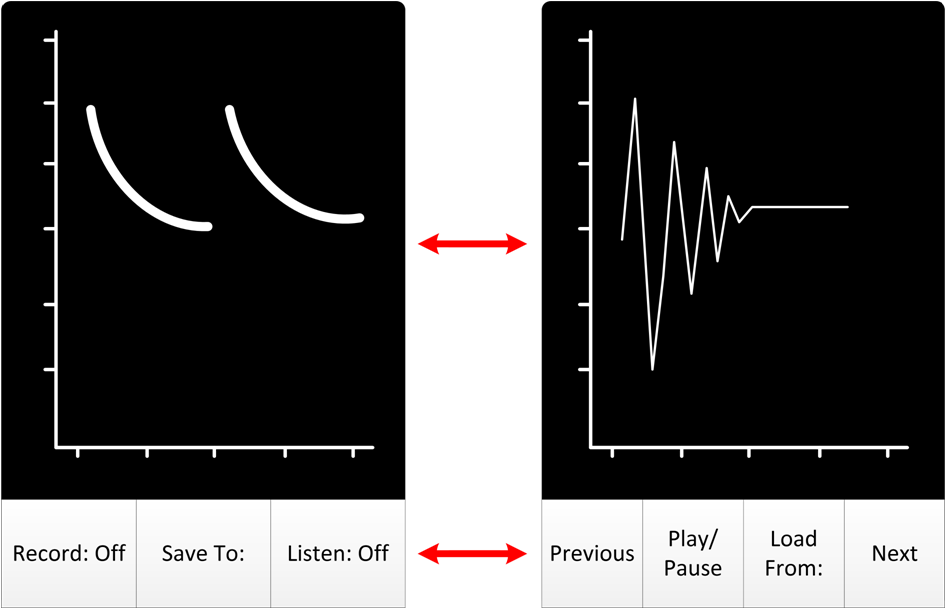
\includegraphics[width=0.4\textwidth]{images/batrec0}
    \hfill
    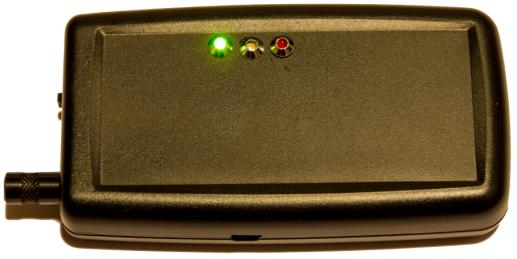
\includegraphics[width=0.4\textwidth]{images/batrec1}
    \graphicscaption{Links: die App, Rechts: das Ger\"at}
}

\fscontent{
    \section{Die Aufgabe}
    Fledermäuse sind nach Angaben des  Bundes vom Aussterben bedroht. Es gilt
    also  diese  seltene  Tierart  vor dem  Aussterben  zu  beschützen. Damit
    dies  überhaupt möglich  ist muss  das Tier  und auch  dessen Lebensraum
    genau-  estens  untersucht  werden. Doch   dies  tönt  einfacher  als  es
    ist. Fledermäuse sind nachtaktiv und ihre Jagd- und Ortungsrufe liegen im
    Ultraschallbereich.

    \section{Die L\"osung}
    
    Es gibt  bereits Geräte die  in der Lage sind  Fledermausrufe aufzunehmen
    und  dann  wiederzugeben.   Das  Problem  liegt  jedoch  darin,  dass  die
    Datenverwaltung nur  auf einem  Computer gemacht werden  kann. Das heisst,
    die  Daten können  nicht  sofort wieder  abgespielt werden. Ein  weiterer
    Punkt  ist  der  Preis. Dieser  ist für  einen  Amateurforscher  viel  zu
    hoch. Hier kommt unser neues Produkt  BatRec ins spiel. Mit BatRec können
    die Ultraschallsignale aufgenommen und auf einem handelsüblichen Android-
    gerät verwaltet und  wiedergegeben werden. Dabei lassen sich  die Rufe im
    Frequenz- oder Zeitbereich analysieren. Es  wurde auf eine Übersichtliche
    und einefache Bedienug fokusiert.

    \section{Die Umsetzung}
    Die  Realisation zu  diesem  bis  anhin nicht  gelösten  Problem ist  ein
    Gerät,  mit  einem  speziellen Ultraschallmikrophon. Um  eine  unnötigen
    Speicherflut zu  vermeiden, wird das Eingangssignal  zuerst gefiltert. Das
    heisst, nur Fledermausartige Signale  von \SI{20}{\kHz} bis \SI{120}{\kHz}
    werden vom  Signalfilter durchgelassen. Anschliessend wird das  Signal vom
    Microcontroller digitalisiert und  anschliessend über eine USB-Verbindung
    an das  Android-Gerät gesendet.  Eine USB-Verbindung  bietet die Vorteile
    von geringerem Akkuverbrauch gegen\"uber Drahtlos-Verbundingen, sowie gute
    \"Ubertragungssicherheit bei ausreichender Geschwindigkeit.

    \section{Die Handhabung}
    All  diese genannten  Forderungen erfüllt  das BatRec. In  einem kleinen,
    handlichen Gehäuse kann  das Gerät an einem  beliebigen Ort positioniert
    werden. Das  Gerät verfügt  über einen  stromsparenden Aufbau,  so kann
    das  gesamte  System ohne  Probleme  zehn  Stunden betrieben  werden. Kurz
    zusammengefasst bietet  das Batrec ein  optimales Tool zum  Aufspüren von
    Fledermäuse, für Profi und Amateur.
}

\infobox{Technischer Aufbau}{%
    \begin{minipage}{0.45\textwidth}
        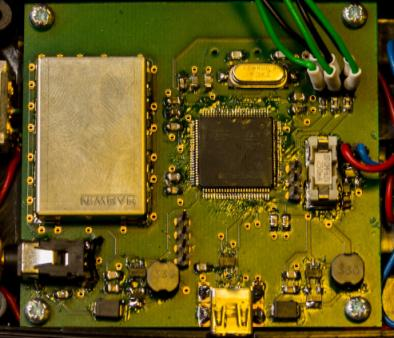
\includegraphics[width=\textwidth]{images/batrec2}
    \end{minipage}
    \hfill
    \begin{minipage}{0.50\textwidth}
        \small
        Die  Hardware wurde  so  kompakt wie  möglich  gemacht.  Dabei  wurde
        darauf geachtet, dass der analoge und der digitale Bereich voneinander
        getrennt wurden. Somit können  grössere Störungen vermieden werden.
        Handhabung und Bedienung wurde möglichst einfach gehalten.
    \end{minipage}
}
